\section{Realisiertes Funktionsmuster}

In diesem Kapitel wird die Umsetzung des in \acrshort{pren1} erarbeiteten Konzept anhand der  erstellten Anforderungsliste bewertet. Der Fokus liegt auf den Fest- und Mindestanforderungen. Die Anforderungsliste ist im Anhang in Kapitel \nameref{anforderungliste} angehängt.

\subsection{Anforderungen}

Die physischen Anforderungen an den Roboter konnten vollständig erfüllt werden. Das maximal zulässige Gewicht von 2 kg wurde mit einem Gesamtgewicht von 1.262 kg, insbesondere durch den Einsatz von Leichtbaustrukturen, deutlich unterschritten. Die maximale Baugrösse 300x300x800mm kann in der Startkonfiguration mit Greifer in Ausgangsstellung eingehalten werden. Zusätzlich erforderliche Komponenten wie ein Notausschalter, ein Eingabetaster zur Zieleingabe sowie eine Statusanzeige wurden erfolgreich integriert.

Die Anforderung 1.6 "Das Fahrzeug muss in der Lage sein das Hindernis mit  einer Masse von 300g anzuheben und im Umkreis von 20mm am alten Ort abzusetzen", konnte nur teilweise erreicht bzw. getestet werden. Der der Anhebemechanismus des Greifers konnte mit dem originalen Hindernis erfolgreich getestet werden. (Siehe Bilder Anheben) Da die Systemintegration jedoch nicht vollständig durchgeführt werden konnte, konnte das Aufheben, Drehen und Absetzen als Prozess nicht getestet werden.

TO DO BILDer GREIFER EINFÜGEN angehoben und offen

Das folgen der Linie erfolgt wie in PREN1 geplant mit einem Liniensensor der aus mehreren Phototransistoren besteht. Die Regelung der Motoren erfolgt mit Hilfe eines PD-Reglers. Der PD-Regler konnte auf dem Testpracour geprüft werden und ist in der Lage der Linie zu folgen und auf einem Knoten anzuhalten. Der Roboter ist auch in der Lage eine bestimmte Distanz zu f

Die Bilderkennung und der Wegfindungsalgorithmus  konnten mithilfe des Kameratestaufbaus aus \acrshort{pren1} und einem leicht veränderten Code bereits vor Ort getestet werden. Gesperrte Knoten konnten bei unseren Testläufen mit einer 100\% Sicherheit erkennt werden, ebenso konnten die Barrieren in 100\% der Fälle erkannt werden. Dies bezieht sich auf die manuellen Testdurchläufe und das Trainingsresultat des Models. Auch die Erkennung der ausgehenden Kanten war immer erfolgreich. Der Algorithmus hat bei allen Testdurchläufen einen direkten Weg ans Ziel gefunden. 

\begin{figure}[H]
\centering
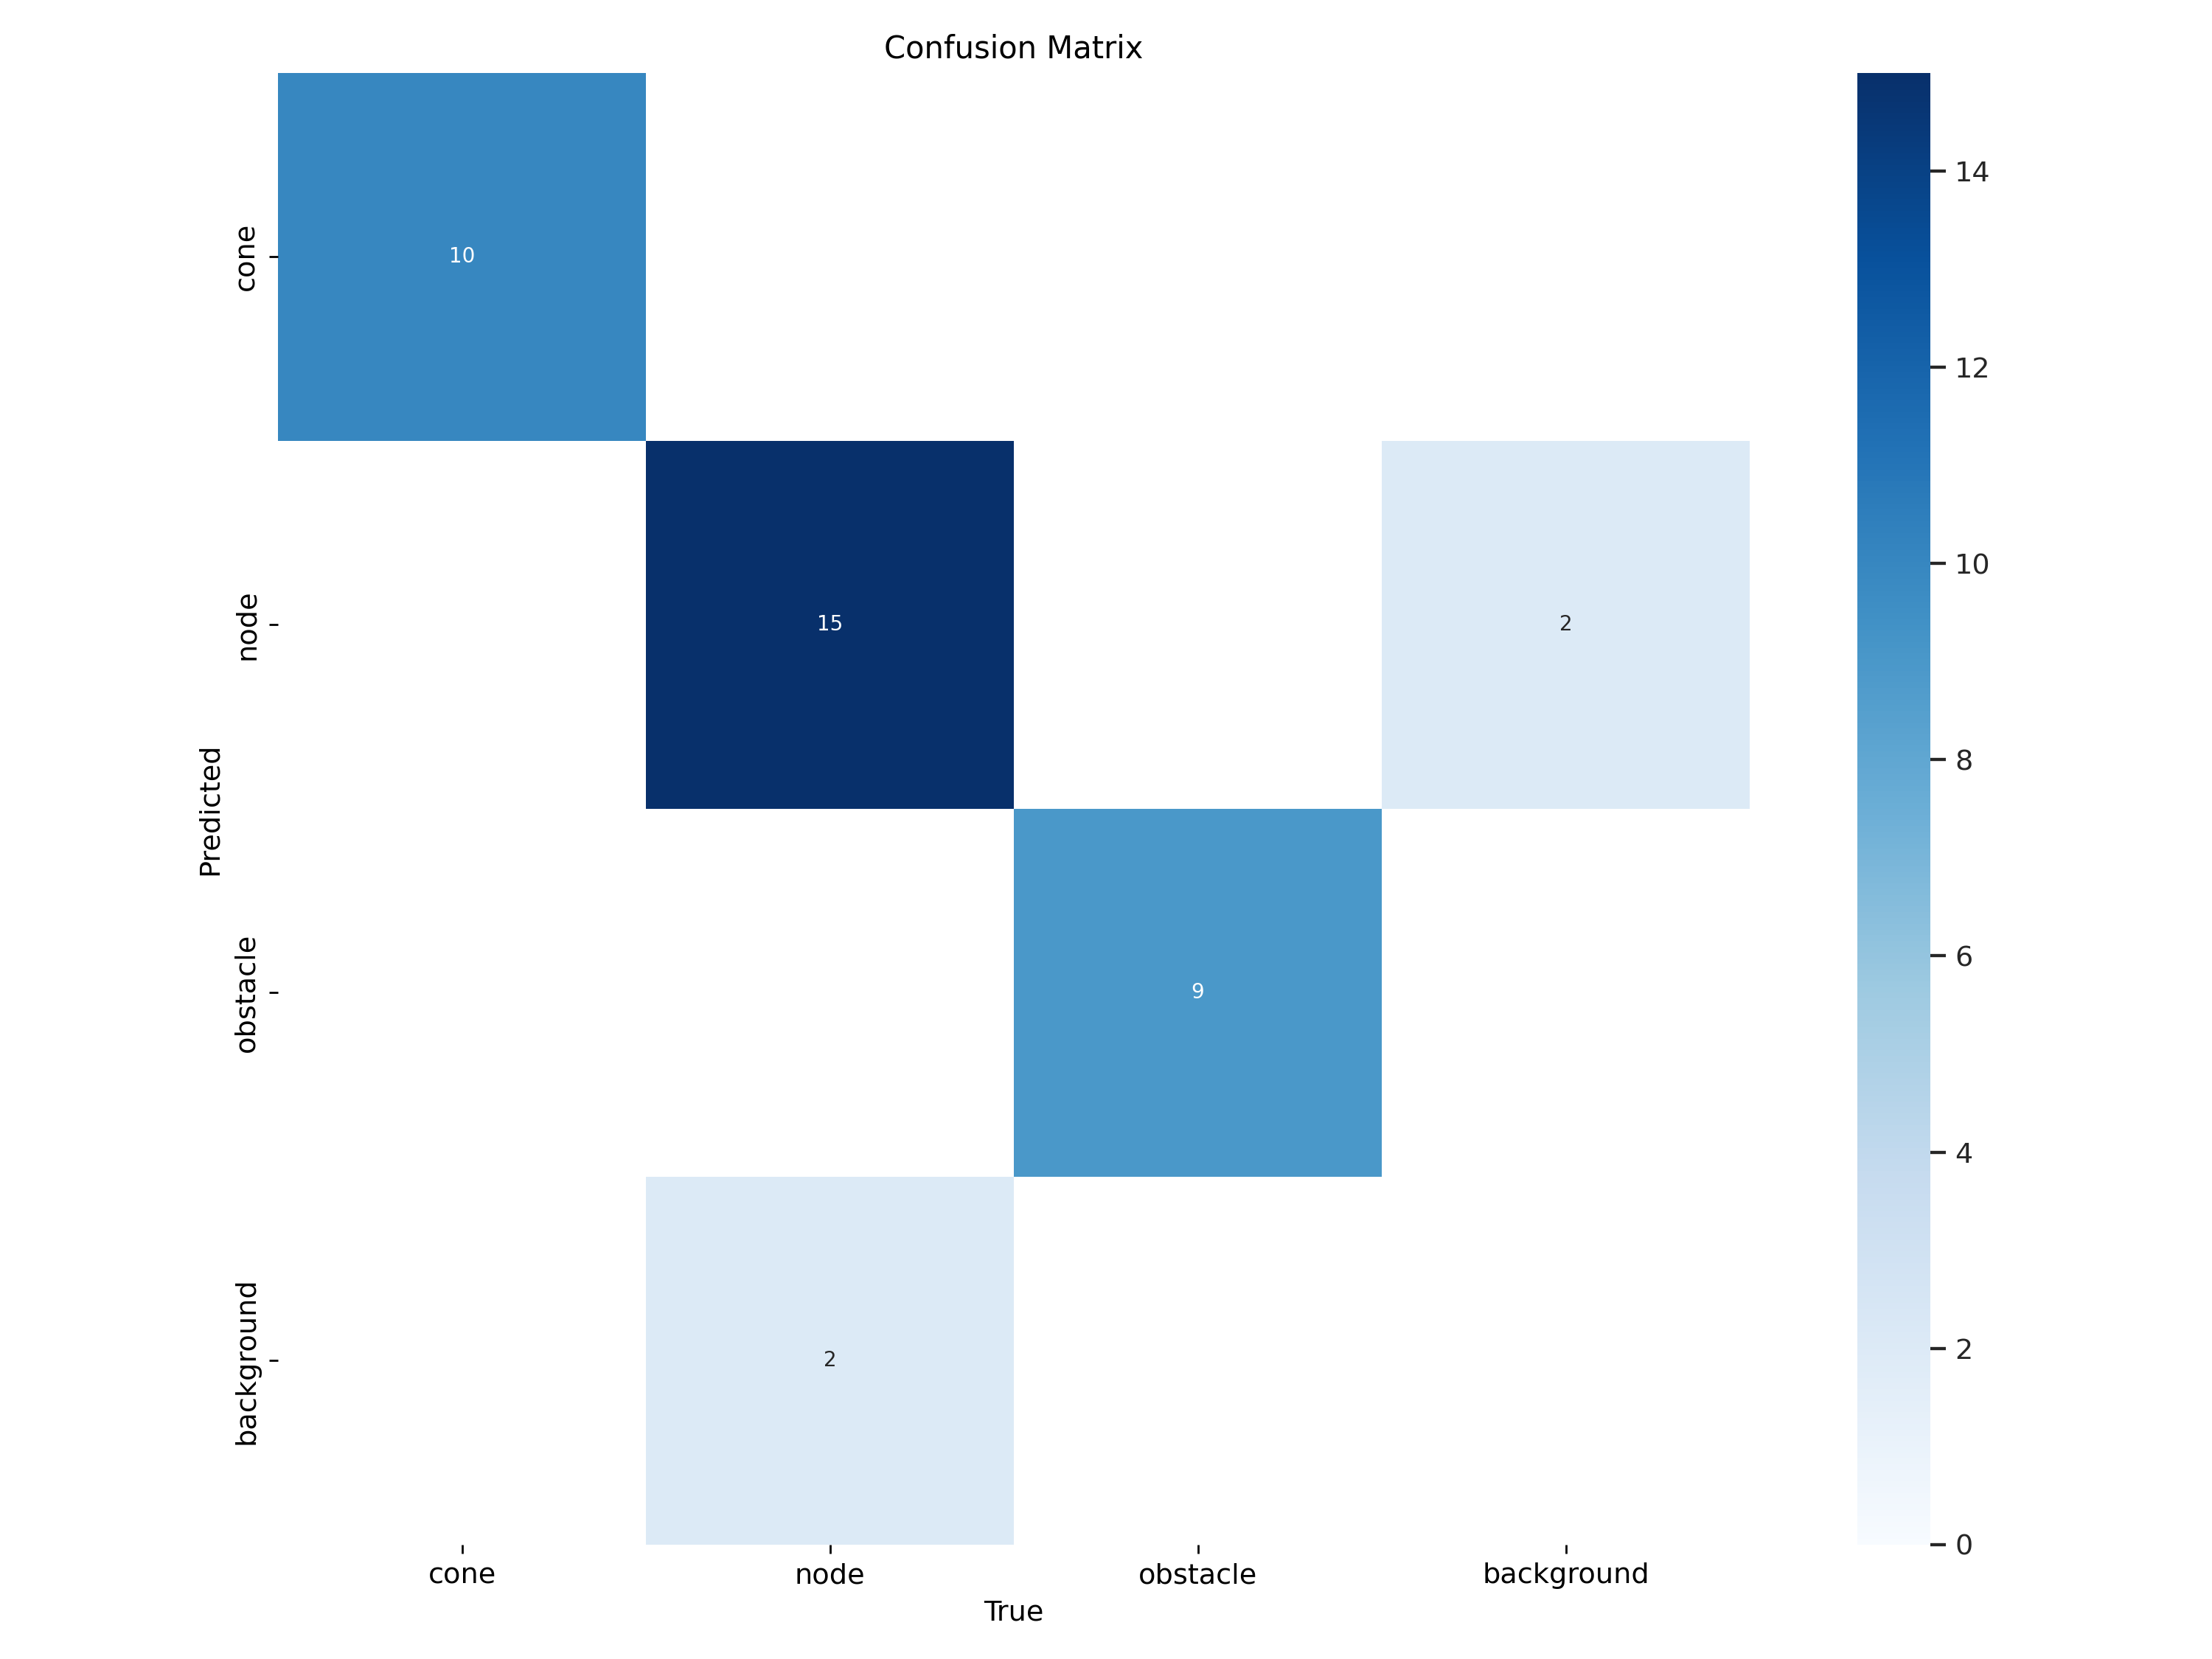
\includegraphics[width=7cm]{assets/IT/yolo/confusion_matrix.png}
\caption{Confusion Matrix Bilderkennung}
\label{fig:conf-matrix-model}
\end{figure}


Die Konstruktionswerkstoffe konnten wie in PREN1 vorgesehen unter Berücksichtigung der im Kapitel Nachhaltigkeit aufgeführten Kriterien ausgewählt werden.